% !TeX spellcheck = cs_CZ
% file: kap_optocoupler.tex
%{\tikzset{external/prefix={tikz/TEO/}}
% \tikzset{external/figure name/.add={ch12_}{}}
%=================== Kapitola: Optoelektronika =====================================================
\setchaptertoc
\chapter{Pasivní elektronické součáskty}\label{teo:IchapXII}


  \section{Teplotní závislost pasivních prvků}\label{teo:IchapXIIsecI}
    
    \begin{example}\label{teo:exam001}
      Uvažujeme žárovku \SI{100}{\watt}, \SI{230}{\volt} s wolframovým vláknem s teplotním 
      součinitelem odporu \(\alpha = \SI{4.8e-3}{\per\kelvin}\).  Problematické je určení provozní 
      teploty vlákna. Vzhledem k tomu, že wolfram taje při teplotě \SI{3387}{\degreeCelsius} a 
      vlákno svítí bílým žárem, odhadneme teplotu na \SI{2500}{\degreeCelsius}. Ze vztahu \(P = 
      U^2/R\) určíme odpor vlákna: \(R = 230^2/100 = \SI{529}{\ohm}\). Odpor při pokojové teplotě 
      bude: 
      \(R_{20}=529/(1+\num{4.8e-3}\cdot2480) = \SI{41}{\ohm}\). 
      \begin{figure}[ht!]  %\ref{teo:fig018}
        \centering
        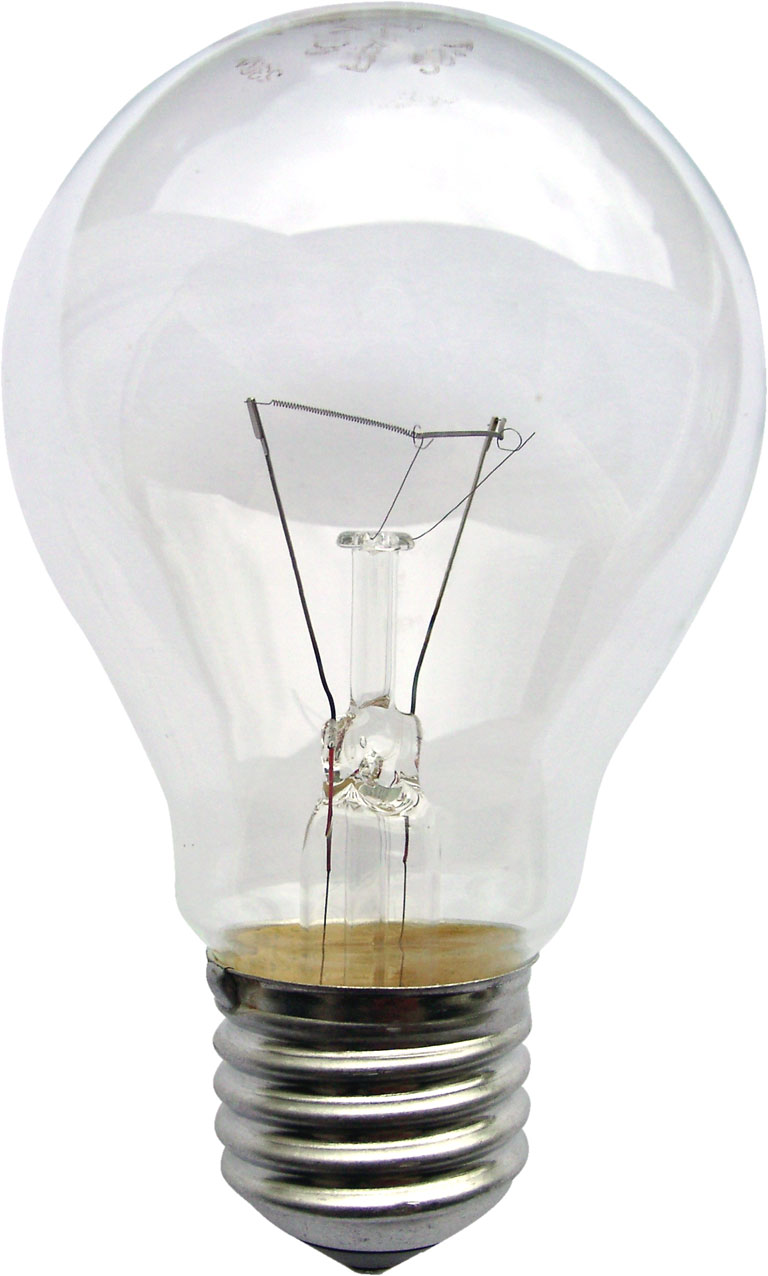
\includegraphics[width=0.3\linewidth]{teo_fig018.jpg}
        \caption{Žárovka jednoduchým způsobem přeměňuje elektrickou energii na světlo, zahříváním 
        tenkého wolframového vodiče průchodem elektrického proudu.}
        \label{teo:fig018}
      \end{figure}
      Podle tohoto přibližného výpočtu se zmenší odpor vlákna  téměř třináctkrát a odpovídajícím 
      způsobem vzrůstá i nárazový proud při zapnutí obvodu oproti ustálenému stavu. Z tohoto 
      pohledu měly původní Edisonovy uhlíkové žárovky lepší vlastnosti, protože teplotní součinitel 
      uhlíku je záporný (\cite[s.~84]{Lanicek1998}).
    \end{example}
%} % tikzset
%---------------------------------------------------------------------------------------------------